%****************************************************************************%
%* Requirements and installation                                            *%
%*                                                                          *%
%* Author(s):                                                               *%
%* - Abdelkader AMAR (Abdelkader.Amar@ens-lyon.fr)                          *%
%* - David LOUREIRO (David.Loureiro@ens-lyon.fr)                            *%
%*                                                                          *%
%* $LICENSE$                                                                *%
%****************************************************************************%
%* $Id: GUM_requirements.tex,v 1.6 2007/11/29 16:03:21 dloureir Exp $
%* $Log: GUM_requirements.tex,v $
%* Revision 1.6  2007/11/29 16:03:21  dloureir
%* typo corrections
%*
%* Revision 1.5  2007/11/28 16:54:07  dloureir
%* Adding the Ganglia module for grudu
%*
%* Revision 1.4  2007/11/28 11:01:38  dloureir
%* Update of the configuration part in the installation section
%*
%* Revision 1.3  2007/11/08 11:31:14  dloureir
%* Correcting the headers
%*
%****************************************************************************%
\chapter{Requirements and installation}

\section{Requirements}

Since \grudu is dedicated to \gfk computing infrastructure, the
first thing you need to use, is a \gfk account and an access to, at
least one site of those composing the platform. For more information about
how to access \gfk, please refer to the web page of \gfk : \url{https://www.grid5000.fr/mediawiki/index.php/Grid5000:Home}

\grudu is written in Java and thus it can be executed on any platform
that offers a recent version of the Java runtime (At least, 1.5.0 version or higher).
Currently, \grudu support only the Bourne shell, so if your \gfk account uses
another shell type, you need to change it. This requirement is only for your \gfk
account and you still can use your preferred shell on your machine.

To allow \grudu to access to all the platform, you need to configure your 
account to authorize a direct access to the different sites. To do so make 
sure all these conditions are fulfilled:

\begin{enumerate}
  \item you have your ssh key in every site: each \gfk site has its own
  NFS filesystem, so you need to copy your ssh key (at least the
  public one) in your \verb|.ssh| directory.
  \item you have you public ssh key in the file
  \verb|$HOME/.ssh/authorized_keys|. You can do this by such a command :
  \verb|cat $HOME/.ssh/id_rsa.pub >> $HOME/.ssh/authorized_keys|.
  \item the following option should be present in your \verb|$HOME/.ssh/config|
  file :\\
  \begin{verbatim}
Host *
StrictHostKeyChecking no
\end{verbatim}
\end{enumerate}

For more information about ssh access to \gfk, key management or file exchange
please refer to the documentation of \gfk at : \url{https://www.grid5000.fr/mediawiki/index.php/Documentation}

\section{Installation}

\subsection{Automatic installation}

\grudu is provided through a single installation jar file containing the GRUDU
software, the required libraries, the source files and the documentation (User
Manual and JavaDoc). This installation file has been created with IzPack\footnote{IzPack is an installer's generator for the Java platform}.

To launch the installer you can either double-click on the installer jar file\footnote{works on operating systems where the jar mime-type is managed by java}
, or launch the jar file from a shell terminal with the following command:\\
\begin{center}
\texttt{java -jar GRUDU\_installer.jar}
\end{center}


The installation is separated into two parts: the installation of the software
itself (the jar file, the libraries and the resource files), and then its
configuration (locally and remotely).

\subsubsection{Installation of the software}

The first one corresponds to the selection of the different ``packages''
you want to install. Five packages are available:
\begin{itemize}
  \item The base package contains the software and the mandatory libraries (It
  is required).
  \item The JFTP module for \grudu. This module corresponds to a File Transfert
  Protocol module. This module allows you to transfert data between \gfk and
  your local machine, but also between the frontales of \gfk. 
  \item The Ganglia module for \grudu. This module corresponds to a plugin
  retrieving data from Ganglia to display low-level information about all the
  nodes of a site or the history of these metrics for the nodes of your jobs.  
  \item The documentation package corresponds to the User's Manual and the JavaDoc of \grudu.
  \item The source code of \grudu.
\end{itemize}
\begin{figure}[H]
\begin{center}
\includegraphics[scale=0.3]{figures/install_packages.eps}
\caption{Installation packages selection}
\end{center}
\end{figure}
If you have an Unix-like operating system (Linux or BSD variants) or
Windows, the seventh panel will allow you to put shortcuts on your desktop and
also in the program group if you want to.\\
\begin{figure}[H]
\begin{center}
\includegraphics[scale=0.3]{figures/install_shortcut.eps}
\caption{Shortcuts configuration}
\end{center}
\end{figure}

\subsubsection{Configuring \grudu}
After having installed \grudu, you should configure it. The
configuration panel is separated into two parts, the first concerns the access
to \gfk. In this tab you have to define :\\
\begin{itemize}
  \item a preferred access point (the external frontal that will be used to
  enter in the \gfk network). The ComboBox contains the different sites of \gfk.
  \item your user name (your \gfk login)
  \item your ssh public key, rsa or dsa (for more information about ssh access
  with public/private keys, please refer to the \gfk Wiki pages treating this subject at :\\
  \url{https://www.grid5000.fr/mediawiki/index.php/SSH}
\end{itemize}
\begin{figure}[H]
\begin{center}
\includegraphics[scale=0.3]{figures/install_configuration.eps}
\caption{\gfk access configuration}
\end{center}
\end{figure}

The second tab of the panel consists in selecting the sites you want
to enable in \grudu (e.g. the sites that will be considered when launching
oarstat or oarnodes commands, or when reserving machines). In this tab you will
also be able to define the partitions used by KaDeploy for the deployment of an
image (for more informations about the partitions you can specify please refer
to the pages of the sites on the \gfk Wiki or to the messages of the day
displayed when you get connected to a site).\\
\begin{figure}[H]
\begin{center}
\includegraphics[scale=0.3]{figures/install_configuration2.eps}
\caption{\gfk clusters configuration}
\end{center}
\end{figure}

When all these information will be filled out, you will be able to write the
configuration by clicking the ``Write configuration'' button. This action will
create the local hierarchy of files mandatory for \grudu (a directory called
\texttt{.diet} containing all the files for \grudu will be created in your home
directory), and the remote hierarchy of files mandatory for \grudu (approximately
the same on the clusters of \gfk).

% \subsection{Automating the installation}
% 
% After having configured GRUDU you can go on to the final panel telling you that
% the installation of GRUDU was successful. An option is proposed for the
% automatic installation of GRUDU on a park of machines. With this file you will
% not have to go through all the installation process by hand and no GUI will be
% shown.\\
% \begin{figure}[H]
% \begin{center}
% \includegraphics[scale=0.3]{figures/GRUDU13.eps}
% \caption{GRUDU remote hierarchy creation}
% \end{center}
% \end{figure}
% To use this file you'll just have to type :
% 
% \begin{verbatim}
% java -jar GRUDU_Installer.jar file_for_automatic_installation.xml
% \end{verbatim}

\subsection{Manual installation}

If you want to compile \grudu sources, you need to install the Java build
tool \textit{Ant}~\footnote{http://ant.apache.org/}. You must have a cvs access
to the \grudu repository. Then simply execute the following command: \verb|ant GRUDU|
 for the compilation. If your login on your local machine differs from the
login on the CVS specify it with the following option : \verb|-Duser=your_cvs_login|

If the compilation succeeds, you will get a new jar file
\textit{GRUDU.jar} representing the program. Launching \grudu can be
done like a typical jar file: \verb|java -jar GRUDU.jar|.

It is preferable that your first step with \grudu is to configure
it. The configuration window contains three tabs, the first corresponding
to the user parameters, the second tab is relative to \gfk sites
and the last one allows you to define specific KaDeploy partitions for the
sites' clusters.

The figure~\ref{fig:cfg_tab1} represents the first tab of the 
configuration windows, where we can found the following parameters:
\begin{itemize}
  \item \textit{Preferred access point}: this is the \gfk site \grudu will
  use to access to all the platform. Your account in this site must
  contain your private ssh key file.
  \item \textit{Username}: your \gfk username.
  \item \textit{Private SSH key file}: your private ssh key file.
\end{itemize}


\begin{figure}[H]
\centering
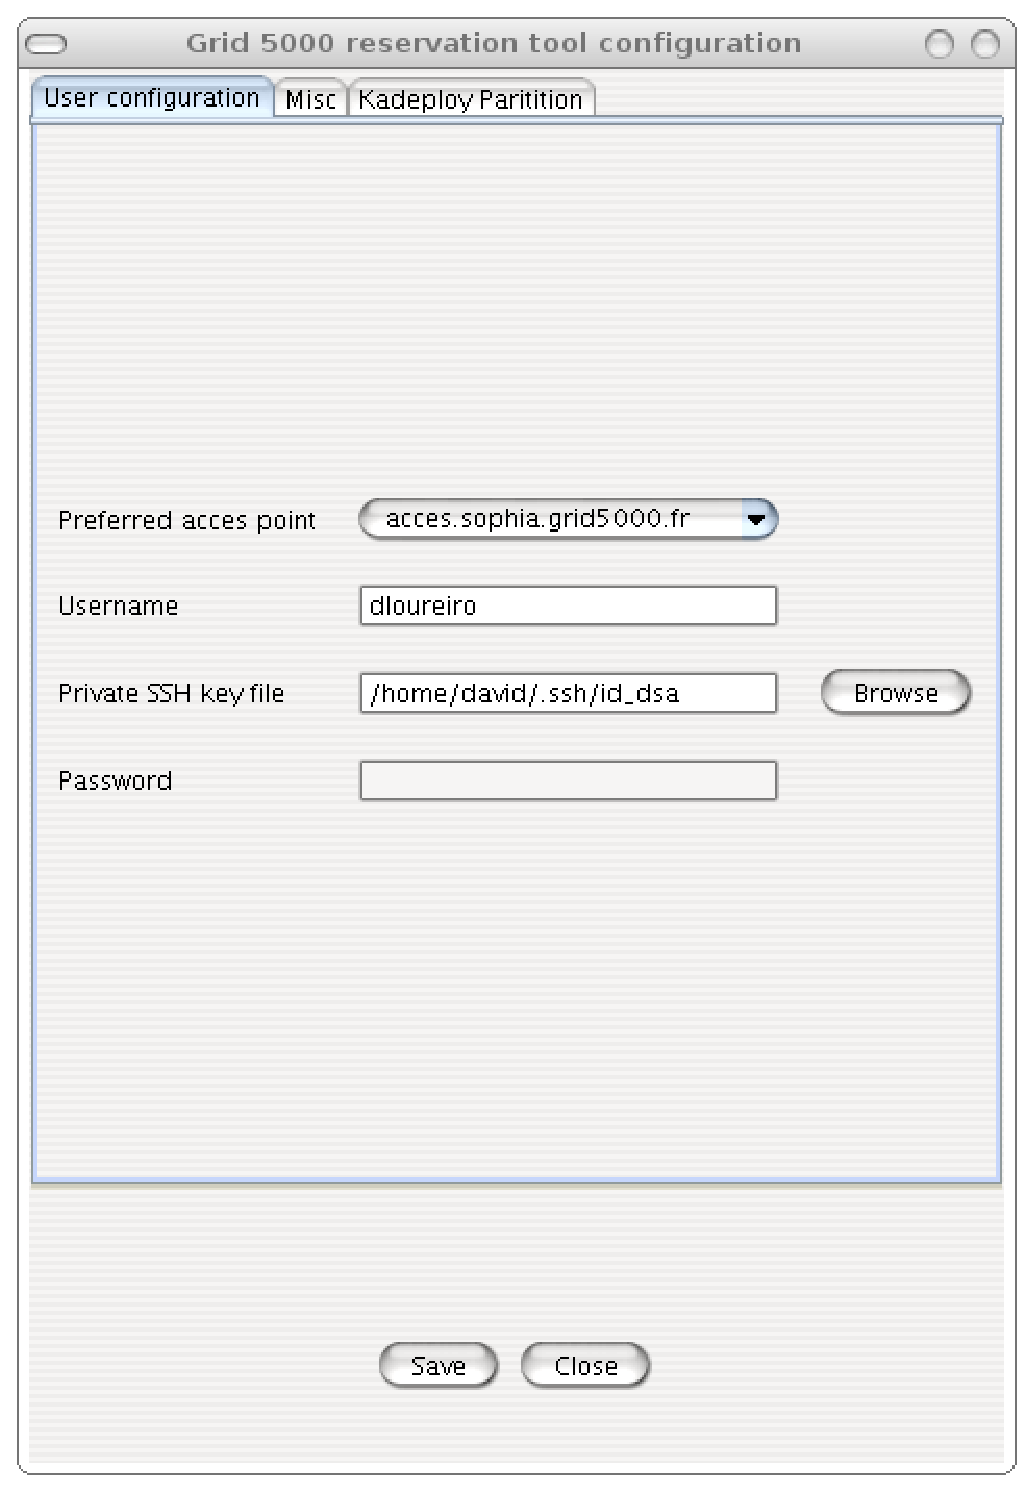
\includegraphics[width=0.4\linewidth]{figures/GRUDU_conf1.eps}
\caption{Configuration window: First tab}
\label{fig:cfg_tab1}
\end{figure}

The second configuration tab shown in figure~\ref{fig:cfg_tab2} allows the user
to configure the following parameters:
\begin{itemize}
  \item Enabling/Disabling a site: by default all sites are disabled.
  \item KaDeploy partition for each site (the same partition will be used for
  every clusters of that site).
  \item OAR batch Scheduler main version (you can choose between oar1 and oar2)
\end{itemize}

\begin{figure}[H]
\centering
\includegraphics[width=0.4\linewidth]{figures/GRUDU_conf2.eps}
\caption{Configuration window: Second tab}
\label{fig:cfg_tab2}
\end{figure}

The third tar shown in figure~\ref{fig:cfg_tab3} allows the user to configure
the KaDeploy partition for every clusters independently.

\begin{figure}[H]
\centering
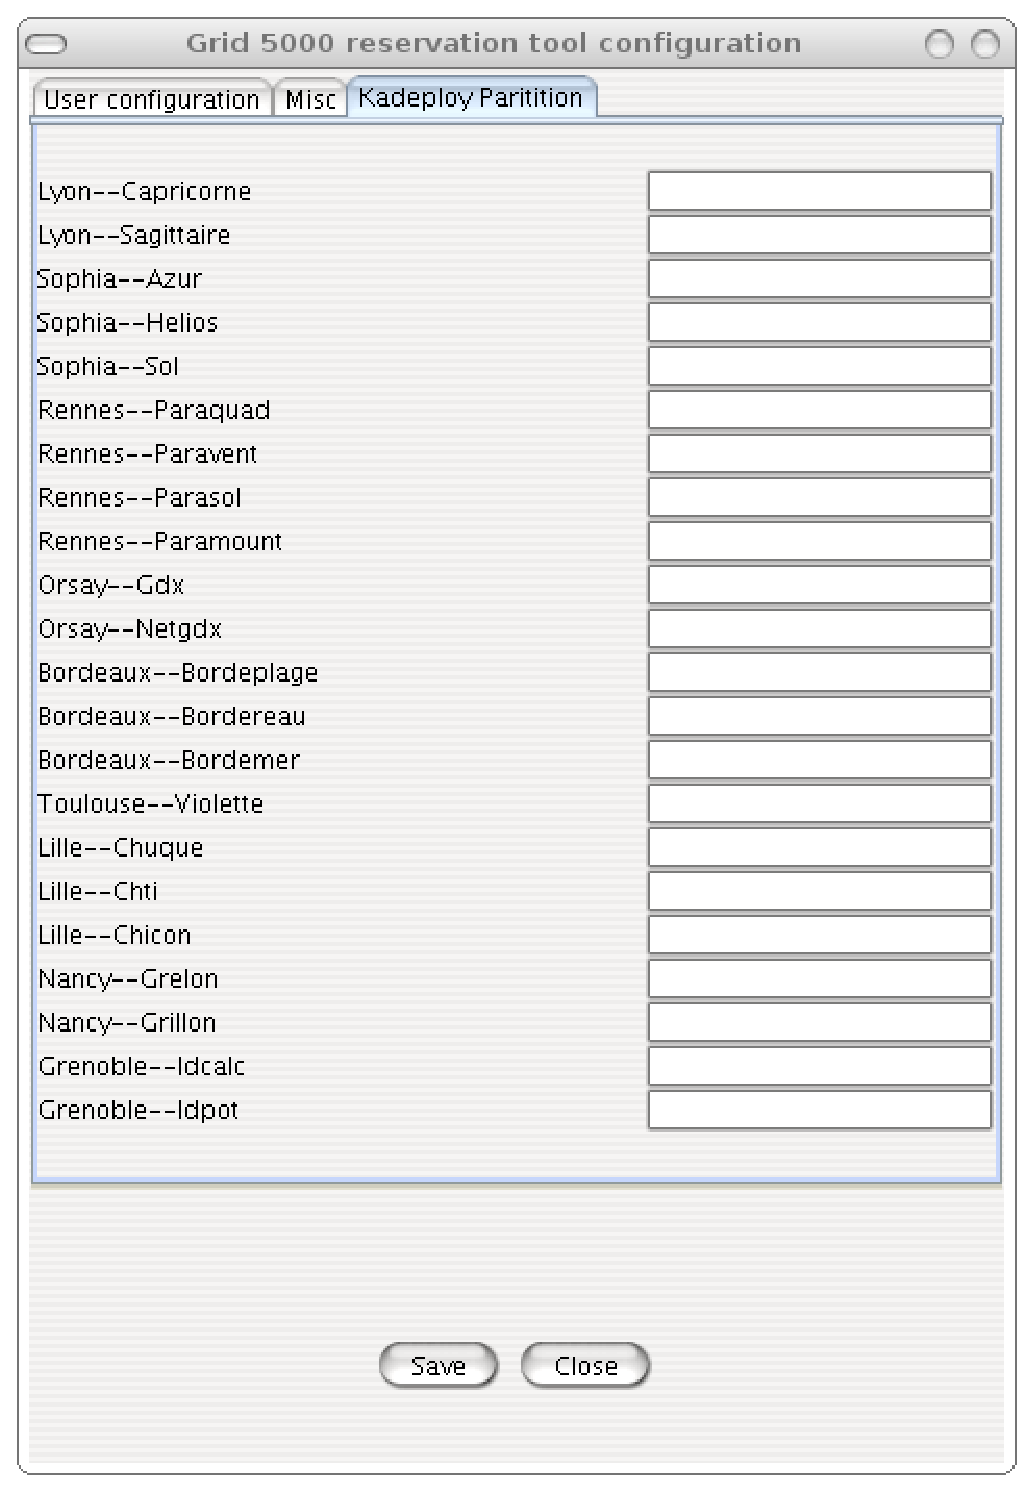
\includegraphics[width=0.4\linewidth]{figures/GRUDU_conf3.eps}
\caption{Configuration window: Third tab}
\label{fig:cfg_tab3}
\end{figure}

%******************************************%